% This is text associated with the open textbook "Open Electromagnetics"
% See immediately below for author, date
% This work is licensed under the Creative Commons Attribution-ShareAlike 4.0 International License. (CC BY-SA 4.0) 
% To view a copy of the license, visit http://creativecommons.org/licenses/by-sa/4.0/

%ORB TITLE Effective Aperture
%ORB AUTHOR 0        # S.W. Ellingson, Virginia Tech (ellingson@vt.edu)
%ORB DATE 20191212   # yyyymmdd
%ORB ABSTRACT 

\label{m0218_Effective_Aperture} % <-- Must match name of this file and module directory name.  Don't mess with this!
\index{effective aperture|(}

When working with systems involving receiving antennas, it is convenient to have a single parameter that relates incident power (as opposed to incident electric field) to the power delivered to the receiver electronics.
This parameter is commonly known as the \emph{effective aperture} or \emph{antenna aperture}. 
\index{antenna aperture}

From elementary circuit theory, the power delivered to a load $Z_L$ is maximized when the load is conjugate matched to the antenna impedance; i.e.,  when $Z_L=Z_A^*$ where $Z_A$ is the impedance of the antenna.
Thus, a convenient definition for effective aperture $A_e$ employs the relationship:
%
\begin{equation}
P_{R,max} \triangleq S^i_{co} A_e
\label{m0218_eAedef}
\end{equation}
%
where 
$S^i_{co}$ is the incident power density (SI base units of W/m$^2$) that is co-polarized with the antenna, and
$P_{R,max}$ is the power delivered to a load that is conjugate matched to the antenna impedance. 
Summarizing:
%
%%%%%%%%%%%%%%%%%%%%%%%%%%%%%%%%%%%%%%%%%%%%%%%
%ORB HIGHLIGHT
\begin{mdframed}[backgroundcolor=yellow!20,nobreak=true] 
\emph{Effective aperture} (SI base units of m$^2$) is the ratio of power delivered by an antenna to a conjugate matched load, to the incident co-polarized power density.
\end{mdframed}
%%%%%%%%%%%%%%%%%%%%%%%%%%%%%%%%%%%%%%%%%%%%%%%

As defined, a method for calculation of effective aperture is not obvious, except perhaps through direct measurement.
In fact, there are at least three ways we can calculate effective aperture: (a) via effective length, (b) via thermodynamics, and (c) via reciprocity.
Each of these methods yields some insight and are considered in turn.

{\bf Effective aperture via effective length.} 
The potential and current at the load of the receive antenna can be determined using the equivalent circuit model shown in Figure~\ref{m0218_AntennaEquivCircuitReception}, using the Th\'{e}venin equivalent circuit model for the antenna developed in Section~\ref{m0206_Equivalent_Circuit_Model_for_Reception}.
%
\begin{figure}[b!] % <--- "[b!]" for first figure in section *only*; delete for 2nd and subsequent figures
\begin{center}
\pdftooltip{{  % note double braces
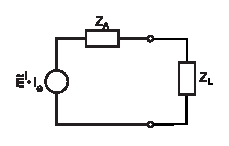
\includegraphics[width=2.5in]{modules/m0218_AntennaEquivCircuitReception.eps} 
% https://en.wikipedia.org/wiki/File:Sidelobes_en.svg
}}{Source labeled capital E tilde superscript small i dot capital i sub small e. This is in series with capital Z sub capital A and capital Z subscript capital L.}
\end{center}
\centerline{\scriptsize 
\copyright~\hyperref[m0216_AntennaEquivCircuitReception_Credit]{S.\ Lally} 
\href{https://creativecommons.org/licenses/by-sa/4.0/}{CC BY-SA 4.0}  
(modified)
} % \centerline 
\caption{
\label{m0218_AntennaEquivCircuitReception}
Equivalent circuit model for an antenna in the presence of an incident electric field $\widetilde{\bf E}^i$, terminated into a load impedance $Z_L$.
}
\end{figure}
%
In this model, the voltage source is determined by the incident electric field intensity $\widetilde{\bf E}^i$ and the vector effective length 
\index{vector effective length}
${\bf l_e}=\hat{\bf l}_el_e$ of the antenna.
We determine the associated effective aperture as follows.
Consider a co-polarized sinusoidally-varying plane wave $\widetilde{\bf E}_{co}^i$ incident on the antenna.
Further, let
%
\begin{equation}
\widetilde{\bf E}_{co}^i = E^i \hat{\bf e}
\end{equation}
%
where $\hat{\bf e}$ is the reference direction of $\widetilde{\bf E}_{co}^i$.
The co-polarized power density incident on the antenna is:
%
\begin{equation}
S^i_{co} = \frac{\left|E^i\right|^2}{2\eta}
\label{m0218_Sico}
\end{equation}
%
where $\eta$ is the wave impedance of the medium (e.g., $\cong 377~\Omega$ for an antenna in free space).
In response, the time-average power delivered to the load is
%
\begin{equation}
P_R = \frac{1}{2}\mbox{Re}\left\{\widetilde{V}_L \widetilde{I}_L^*\right\}
\label{m0218_ePA1}
\end{equation}
%
where $\widetilde{V}_L$ and $\widetilde{I}_L$ are the potential and current phasors, respectively, at the load.
%
We may determine $\widetilde{V}_L$ and $\widetilde{I}_L$ from the equivalent circuit model of Figure~\ref{m0218_AntennaEquivCircuitReception} using basic circuit theory.
First, note that the magnitude and phase of the voltage source is:
%
\begin{equation}
\widetilde{\bf E}_{co}^i \cdot {\bf l}_e = E^i l_e \left( \hat{\bf e} \cdot \hat{\bf l}_e \right)
\end{equation}
%
and since we have defined $\hat{\bf l}_e$ to be equal to $\hat{\bf e}$,
%
\begin{equation}
\widetilde{\bf E}_{co}^i \cdot {\bf l}_e = E^i l_e 
\end{equation}
%
Next, note that the load impedance creates a voltage divider with the source (antenna) impedance such that 
%
\begin{equation}
\widetilde{V}_L = \left( E^i l_e \right) \frac{Z_L}{Z_A+Z_L}
\end{equation}
%
Similarly, $\widetilde{I}_L$ is the voltage source output divided by the total series resistance: 
%
\begin{equation}
\widetilde{I}_L = \frac{E^i l_e }{Z_A+Z_L}
\end{equation}
%
Substituting these expressions into Equation~\ref{m0218_ePA1}, we obtain:
%
\begin{equation}
P_R = \frac{1}{2} \left|E^i l_e \right|^2 \frac{R_L}{\left|Z_A+Z_L\right|^2} 
\end{equation}
%
Let us identify the real and imaginary components of $Z_A$ and $Z_L$ explicitly, as follows:
%
\begin{equation}
Z_A = R_A +jX_A
\end{equation}
%
\begin{equation}
Z_L = R_L +jX_L
\end{equation}
%
Further, let us assume that loss internal to the antenna is negligible, so $R_A \approx R_{rad}$.
If $Z_L$ is conjugate matched for maximum power transfer, then $Z_L=Z_A^*=R_{rad}-jX_A$.
Therefore:
%
\begin{flalign}
P_{R,max} &= \frac{1}{2} \left|E^i l_e \right|^2 \frac{R_{rad}}{\left|Z_A+Z_A^*\right|^2} \nonumber \\
          &= \frac{1}{2} \left|E^i l_e \right|^2 \frac{R_{rad}}{\left|2R_{rad}\right|^2} \nonumber \\
          &= \frac{\left|E^i l_e \right|^2}{8R_{rad}} \label{m0219_PRmax}
\end{flalign}

Now using Equations~\ref{m0218_eAedef}, \ref{m0218_Sico}, and \ref{m0219_PRmax}, we find:
%
\begin{equation}
A_e = \frac{\left|E^i l_e \right|^2 / 8R_{rad} }{ \left|E^i\right|^2 / 2\eta  } 
\end{equation}
%
which reduces to:
%
\begin{equation}
\boxed{
A_e = \frac{ \eta \left|l_e\right|^2 }{ 4 R_{rad} } 
}
\label{m0218_eAeel}
\end{equation}

It is not surprising that effective aperture should be proportional to the square of the magnitude of effective length.
However, we see that the medium and the radiation resistance of the antenna also play a role.

%Be warned that Equation~\ref{m0218_eAeel} often appears in the literature without the factor of $\cos^2\psi$. In some cases, this is because the \emph{maximum} value of $A_e$ is desired, so $\psi=0$ is assumed. In other cases, this is because ``vector effective length'' \index{vector effective length} has been defined to be aligned with the incident electric field, so $\psi$ is always equal to $0$; see Section~\ref{m0206_Equivalent_Circuit_Model_for_Reception} for additional information about this particular issue.

Effective length and radiation resistance are easy to calculate for wire antennas, so it is natural to use Equation~\ref{m0218_eAeel} to calculate the effective apertures of wire antennas.
For the electrically-short dipole (ESD)
\index{antenna!electrically-short dipole (ESD)}
of length $L$, $l_e\approx(L/2)\sin\theta$ and $R_{rad} \approx 20\pi^2\left(L/\lambda\right)^2$.
Thus, we find the effective aperture assuming free space (i.e., $\eta=\eta_0$) is:
%
\begin{equation}
A_e \approx 0.119\lambda^2 \left|\sin\theta\right|^2 ~~~\mbox{(lossless ESD)}
\end{equation}
%
Remarkably, the effective aperture of the ESD does not depend on its length.
In fact, it depends only on the frequency of operation.

Also worth noting is that \emph{maximum} effective aperture (i.e., the effective aperture in the $\theta=\pi/2$ direction) is
%
\begin{equation}
\boxed{ A_e \approx 0.119\lambda^2 } ~~~\mbox{(lossless ESD, max.)}
\end{equation}

Dipoles which are not electrically-short exhibit radiation resistance which is proportional to $L^p$, where $p>2$.
Therefore, the effective aperture of non-electrically-short dipoles \emph{does} increase with $L$, as expected.
However, this increase is not dramatic unless $L$ is significantly greater than $\lambda/2$.
Here's an example:

%%%%%%%%%%%%%%%%%%%%%%%%%%%%%%%%%%%%%%%%%%%%%%%
%ORB EXAMPLE
~\\ \begin{example} 
\begin{mdframed}[backgroundcolor=brown!20,linecolor=brown!20]\raggedright
Effective aperture of a half-wave dipole.
\index{antenna!half-wave dipole}
\\~\\
The electrically-thin half-wave dipole exhibits radiation resistance $\cong 73~\Omega$ and effective length $\lambda/\pi$.
Assuming the dipole is lossless and in free space, Equation~\ref{m0218_eAeel} yields:
%
\begin{equation}
A_e \approx 0.131\lambda^2 ~~~\mbox{(half-wave dipole, max.)}
\end{equation}
%
Again, this is the effective aperture for a wave incident from broadside to the dipole.
\end{mdframed}
% note figures will need to go between "\end{mdframed}" and "\end{example}"
\end{example}
%%%%%%%%%%%%%%%%%%%%%%%%%%%%%%%%%%%%%%%%%%%%%%%

{\bf Effective aperture via thermodynamics.}
\index{thermodynamics}
A useful insight into the concept of effective aperture can be deduced by asking the following question:
How much power is received by an antenna when waves of equal power density arrive from all directions simultaneously?
This question is surprisingly easy to answer using basic principles of thermodynamics.
Thermodynamics is a field of physics that addresses heat and its relation to radiation and electrical energy.
No previous experience with thermodynamics is assumed in this derivation. 

Consider the scenario depicted in Figure~\ref{m0218_fThermo}.
%
\begin{figure}[b!] % <--- "[b!]" for first figure in section *only*; delete for 2nd and subsequent figures
%
\begin{center}
\pdftooltip{{  % note double braces
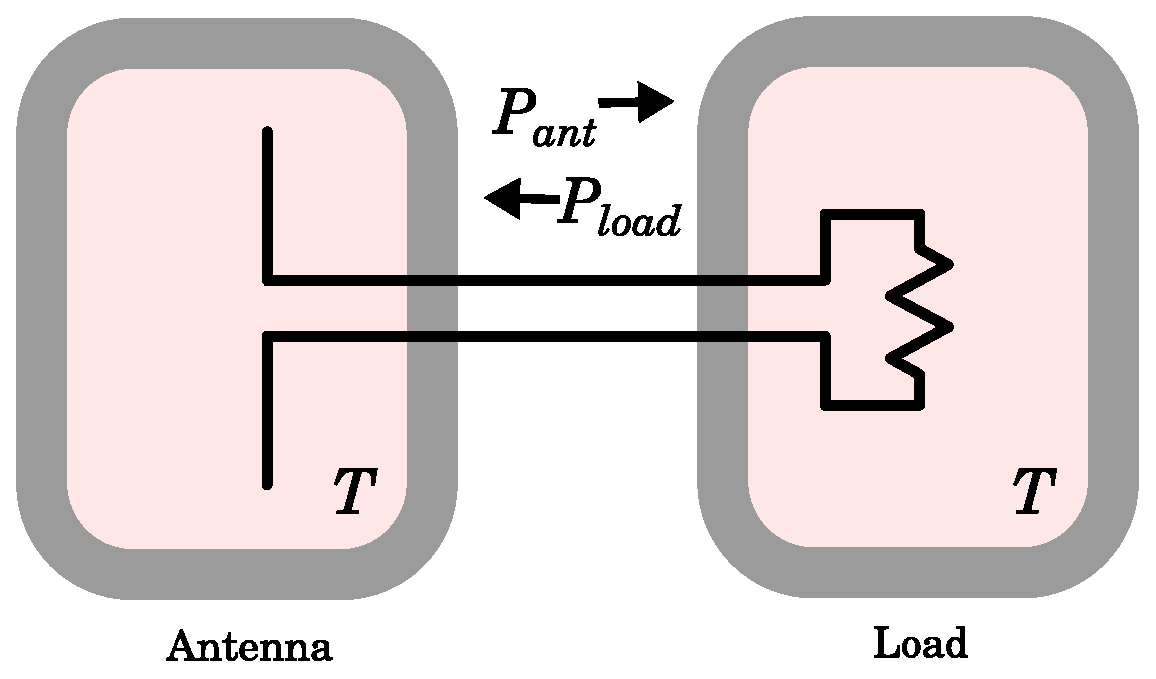
\includegraphics[width=2.5in]{modules/m0218_fThermo.eps} 
% https://en.wikipedia.org/wiki/File:Antenna_and_resistor_in_cavity.svg
}}{Two rounded rectangular regions, labeled Antenna (left) and Load (right). Both have an interior region labeled capital T. Arrow pointing from Antenna to Load is capital P subscript ant. Arrow pointing from load to antenna is capital P subscript load.  A wire begins in Antenna, goes to Load where it goes through a resistor, and comes back into the Antenna capital T region.}
\end{center}
\centerline{\scriptsize 
\hyperref[m0218_fThermo_Credit]{Chetvorno}, 
public domain
(modified) 
} % \centerline 
\caption{
\label{m0218_fThermo}
Thermodynamic analysis of the power exchanged between an antenna and its load.
}
\end{figure}
%
In this scenario, the antenna is completely enclosed in a chamber whose walls do not affect the behavior of the antenna and which have uniform temperature $T$.
The load (still conjugate matched to the antenna) is completely enclosed by a separate but identical chamber, also at temperature $T$.

Consider the load chamber first.  
Heat causes random acceleration of constituent charge carriers in the load, giving rise to a randomly-varying current at the load terminals.  
(This is known as \emph{Johnson-Nyquist noise}.)
\index{Johnson-Nyquist noise}
This current, flowing through the load, gives rise to a potential; therefore, the load -- despite being a passive device -- is actually a source of power. 
The power associated with this noise is:
%
\begin{equation}
P_{load} = kTB
\label{m0218_ePload}
\end{equation}
%
where 
$k\cong 1.38 \times 10^{-23}$~J/K is \emph{Boltzmann's constant}
\index{Boltzmann's constant}
and $B$ is the bandwidth within which $P_{load}$ is measured.

Similarly, the antenna is a source of noise power $P_{ant}$.
$P_{ant}$ can also be interpreted as captured \emph{thermal radiation} --
\index{thermal radiation} 
that is, electromagnetic waves stimulated by the random acceleration of charged particles comprising the chamber walls.
These waves radiate from the walls and travel to the antenna.
The \emph{Rayleigh-Jeans law} 
\index{Rayleigh-Jeans law}
of thermodynamics tells us that this radiation should have power density (i.e., SI base units of W/m$^2$) equal to 
%
\begin{equation}
\frac{2kT}{\lambda^2}~B
\end{equation}
%
per steradian of solid angle.\footnote{Full disclosure: This is an approximation to the exact expression, but is very accurate at radio frequencies.  See ``Additional Reading'' at the end of this section for additional details.}
The total power accessible to the antenna is one-half this amount, since an antenna is sensitive to only one polarization at a time, whereas the thermal radiation is equally distributed among any two orthogonal polarizations.
$P_A$ is the remaining power, obtained by integrating over all $4\pi$ steradians.
Therefore, the antenna captures total power equal to\footnote{Recall $\sin\theta' d\theta' d\phi'$ is the differential element of solid angle.}
%
\begin{flalign}
P_{ant} &= \oint { A_e(\theta',\phi') \left(\frac{1}{2}~\frac{2kT}{\lambda^2}~B \right) \sin\theta' d\theta' d\phi'  } \nonumber \\
        &= \left(\frac{kT}{\lambda^2}~B \right) \oint { A_e(\theta',\phi') \sin\theta' d\theta' d\phi'  } \label{m0218_ePant}
\end{flalign}

Given the conditions of the experiment, and in particular since the antenna chamber and the load chamber are at the same temperature, the antenna and load are in \emph{thermodynamic equilibrium}.
\index{thermodynamic equilibrium}
A consequence of this equilibrium is that power $P_{ant}$ captured by the antenna and delivered to the load must be equal to power $P_{load}$ generated by the load and delivered to the antenna; i.e., 
%
\begin{equation}
P_{ant} = P_{load} 
\label{m0218_eTE}
\end{equation}
%
Combining Equations~\ref{m0218_ePload}, \ref{m0218_ePant}, and \ref{m0218_eTE}, we obtain:
%
\begin{equation}
\left(\frac{kT}{\lambda^2}~B \right) \oint { A_e(\theta',\phi') \sin\theta' d\theta' d\phi'  } = kTB
\end{equation}
%
which reduces to:
%
\begin{equation}
\oint { A_e(\theta',\phi') \sin\theta' d\theta' d\phi'  } = \lambda^2
\label{m0218_fAT1}
\end{equation}

Let $\left<A_e\right>$ be the \emph{mean} effective aperture of the antenna; i.e., $A_e$ averaged over all possible directions.
This average is simply Equation~\ref{m0218_fAT1} divided by the $4\pi$~sr of solid angle comprising all possible directions.  Thus:
%
\begin{equation}
\left<A_e\right> = \frac{\lambda^2}{4\pi}
\end{equation}

Recall that a \emph{isotropic} antenna
\index{antenna!isotropic}
is one which has the same effective aperture in every direction.
Such antennas do not exist in practice, but the concept of an isotropic antenna is quite useful as we shall soon see.
Since the effective aperture of an isotropic antenna must be the same as its mean effective aperture, we find:  
%
\begin{equation}
\boxed{
A_e = \frac{\lambda^2}{4\pi} \approx 0.080\lambda^2 ~~~\mbox{(isotropic antenna)}
}
\end{equation}
%
Note further that this must be the \emph{minimum possible} value of the maximum effective aperture for \emph{any} antenna.

{\bf Effective aperture via reciprocity.}
The fact that all antennas have maximum effective aperture greater than that of an isotropic antenna makes the isotropic antenna a logical benchmark against which to compare the effective aperture of antennas.
We can characterize the effective aperture of any antenna as being some unitless real-valued constant $D$ times the effective aperture of an isotropic antenna; i.e.:
%
\begin{equation}
\boxed{
A_e \triangleq D \frac{\lambda^2}{4\pi} ~~~\mbox{(any antenna)}
}
\label{m0218_eAe1}
\end{equation}
%
where $D$ must be greater than or equal to 1.

Astute readers might notice that $D$ seems a lot like \emph{directivity}.
\index{directivity}
Directivity is defined in Section~\ref{m0203_Directivity_and_Gain} as the factor by which a \emph{transmitting} antenna increases the power density of its radiation over that of an isotropic antenna.
Let us once again consider the ESD, for which we previously determined (via the effective length concept) that $A_e\cong 0.119\lambda^2$ in the direction in which it is maximum.
Applying Equation~\ref{m0218_eAe1} to the ESD, we find:
%
\begin{equation}
D \triangleq A_e \frac{4\pi}{\lambda^2}  \cong 1.50 ~~~\mbox{(ESD, max.)}
\end{equation}
%
Sure enough, $D$ is equal to the directivity of the ESD in the transmit case.

This result turns out to be generally true; that is:
%
%%%%%%%%%%%%%%%%%%%%%%%%%%%%%%%%%%%%%%%%%%%%%%%
%ORB HIGHLIGHT
\begin{mdframed}[backgroundcolor=yellow!20,nobreak=true] 
The effective aperture of \emph{any} antenna is given by Equation~\ref{m0218_eAe1} where $D$ is the directivity of the antenna when transmitting.
\end{mdframed}
%%%%%%%%%%%%%%%%%%%%%%%%%%%%%%%%%%%%%%%%%%%%%%%
%
A derivation of this result for the general case is possible using analysis similar to the thermodynamics presented earlier, or using the reciprocity theorem developed in Section~\ref{m0214_Reciprocity}.

The fact that effective aperture is easily calculated from transmit directivity is an enormously useful tool in antenna engineering.
Without this tool, determination of effective aperture is limited to direct measurement or calculation via effective length; and effective length is generally difficult to calculate for antennas which are not well-described as distributions of current along a line.
It is usually far easier to calculate the directivity of an antenna when transmitting, and then use Equation~\ref{m0218_eAe1} to obtain effective aperture for receive operation.

Note that this principle is itself an expression of reciprocity.
That is, one may fairly say that ``directivity'' is not exclusively a transmit concept nor a receive concept, but rather is a single quantifiable characteristic of an antenna that applies in both the transmit and receive case.
Recall that radiation patterns 
\index{pattern (radiation)}
are used to quantify the way (transmit) directivity varies with direction.
Suddenly, we have found that precisely the same patterns apply to the receive case!
Summarizing:
%
%%%%%%%%%%%%%%%%%%%%%%%%%%%%%%%%%%%%%%%%%%%%%%%
%ORB HIGHLIGHT
\begin{mdframed}[backgroundcolor=yellow!20,nobreak=true] 
As long as the conditions required for formal reciprocity are satisfied, the directivity of a receiving antenna (defined via Equation~\ref{m0218_eAe1}) is equal to directivity of the same antenna when transmitting, and patterns describing receive directivity are equal to those for transmit directivity.
\end{mdframed}
%%%%%%%%%%%%%%%%%%%%%%%%%%%%%%%%%%%%%%%%%%%%%%%

Finally, we note that the equivalence of transmit and receive directivity can, again via Equation~\ref{m0218_eAe1}, be used to define an effective aperture for the transmit case.
In other words, we can define the effective aperture of a transmitting antenna to be $\lambda^2/4\pi$ times the directivity of the antenna.
There is no new physics at work here; we are simply taking advantage of the fact that the concepts of effective aperture and directivity describe essentially the same characteristic of an antenna, and that this characteristic is the same for both transmit and receive operation.

%%%%%%%%%%%%%%%%%%%%%

{\bf Additional Reading:}
\begin{itemize}
\item ``\href{https://en.wikipedia.org/wiki/Antenna_aperture}{Antenna aperture}'' on Wikipedia.
\item ``\href{https://en.wikipedia.org/wiki/Boltzmann_constant}{Boltzmann constant}'' on Wikipedia.
\item ``\href{https://en.wikipedia.org/wiki/Rayleigh%E2%80%93Jeans_law}{Rayleigh-Jeans law}'' on Wikipedia.
\item ``\href{https://en.wikipedia.org/wiki/Johnson%E2%80%93Nyquist_noise}{Johnson-Nyquist noise}'' on Wikipedia.
\item ``\href{https://en.wikipedia.org/wiki/Thermodynamics}{Thermodynamics}'' on Wikipedia.
\end{itemize}

%%%%%%%%%%%%%%%%%%%%%%

\index{effective aperture|)}

